\documentclass[12pt]{article}
\usepackage[utf8]{inputenc}
\usepackage{amsmath}
\usepackage{amsfonts}
\usepackage{amssymb}
\usepackage{graphicx}
\usepackage{float}
\usepackage{geometry}
\usepackage{listings}
\usepackage{xcolor}
\usepackage{booktabs}
\usepackage{multirow}
\usepackage{subcaption}

\geometry{margin=1in}

\lstset{
    basicstyle=\ttfamily\small,
    keywordstyle=\color{blue},
    commentstyle=\color{gray},
    stringstyle=\color{red},
    numbers=left,
    numberstyle=\tiny,
    frame=single,
    breaklines=true,
    language=Python
}

\title{\textbf{IE 708: Quiz 2 Numerical Solution}}
\author{Dhairya Kantawala (23B3321) \\ Department of Mathematics \\ Indian Institute of Technology Bombay}
\date{\today}

\begin{document}

\maketitle

\section{Introduction}

This report presents the implementation and analysis of an Age of Information (AOI) Markov Decision Process (MDP). The problem models a system where a central controller (CC) utilizes information from two sources to complete jobs. In each time slot, the CC can request an update from at most one source. Each update attempt succeeds independently with probability $q$ ($0 < q < 1$), and new updates are only available at the end of the slot. When a request for update is successful for source $i$, the age of source $i$ becomes 0 while the other source's age becomes $j + 1$. The system incurs a cost $\sigma$ when requesting updates (action $a \neq 0$), with no cost for the "do nothing" action ($a = 0$). The reward function $f(x_1, x_2)$ models the value of information based on the current ages of both sources.

\section{MDP Formulation}

\subsection{State Space}
The state space $\mathcal{S}$ is defined as:
$$\mathcal{S} = \{0, 1, \ldots, L\} \times \{0, 1, \ldots, L\}$$
where each state $(i, j) \in \mathcal{S}$ represents the age of information from two sources, with $i, j \in \{0, 1, \ldots, L\}$ for maximum age $L = 3$.

\subsection{Action Space}
The action space $\mathcal{A} = \{0, 1, 2\}$ represents three possible actions:
\begin{itemize}
    \item Action 0: Do nothing (wait)
    \item Action 1: Query source 1
    \item Action 2: Query source 2
\end{itemize}

\subsection{Reward Function}
The reward function $R: \mathcal{S} \times \mathcal{A} \rightarrow \mathbb{R}$ is defined as:
$$R(i, j, a) = \begin{cases}
f(i, j) & \text{if } a = 0 \\
f(i, j) - \sigma & \text{if } a = 1, 2
\end{cases}$$

where $f(i, j) = e^{-\eta i - j}$ for $i < L$ and $j < L$, and $f(i, j) = 0$ otherwise.

Here:
\begin{itemize}
    \item $\eta > 0$ is the decay parameter for source 1
    \item $\sigma \geq 0$ is the query cost
    \item The function $f(i, j)$ represents the value of information at age $(i, j)$
\end{itemize}

\subsection{Transition Probabilities}
The transition probabilities $T(s'|s, a)$ are defined as follows:

For states $(i, j)$ where $i < L$ and $j < L$:
\begin{align}
T(i+1, j+1 | i, j, 0) &= 1 \\
T(i+1, j+1 | i, j, 1) &= 1 - q \\
T(i+1, 0 | i, j, 1) &= q \\
T(i+1, j+1 | i, j, 2) &= 1 - q \\
T(0, j+1 | i, j, 2) &= q
\end{align}

For boundary states where $i = L$ or $j = L$, the transitions follow similar patterns but respect the maximum age constraint $L$.

Here, $q \in [0, 1]$ represents the probability of successful query (information refresh).

\section{Implementation}

\subsection{Policy Iteration Algorithm}
The optimal policy is computed using policy iteration with the following steps:

\begin{enumerate}
    \item Initialize policy $d^{(0)}$
    \item \textbf{Policy Evaluation}: For current policy $d^{(k)}$, solve:
    $$V^{(k)} = R^{(k)} + \lambda P^{(k)} V^{(k)}$$
    where $\lambda$ is the discount factor.
    
    \item \textbf{Policy Improvement}: Update policy:
    $$d^{(k+1)}(s) = \arg\max_{a} \left[ R(s, a) + \lambda \sum_{s'} T(s'|s, a) V^{(k)}(s') \right]$$
    
    \item Repeat until convergence: $d^{(k+1)} = d^{(k)}$
\end{enumerate}

\subsection{Code Implementation}

\subsubsection{Core MDP Class Structure}
\begin{lstlisting}[caption=Core MDP Class Structure]
class AgoOfInformation:
    def __init__(self, L, eta, sigma, q):
        self.L = L
        self.eta = eta
        self.sigma = sigma
        self.q = q
        
        # Initialize reward and transition matrices
        self.rewards = np.zeros((self.L+1, self.L+1, 3))
        self.transitions = np.zeros((self.L+1, self.L+1, self.L+1, self.L+1, 3))
        
        # Build reward matrix
        for i in range(self.L+1):
            for j in range(self.L+1):
                self.rewards[i, j, 0] = f(i, j)
                self.rewards[i, j, 1] = f(i, j) - self.sigma
                self.rewards[i, j, 2] = f(i, j) - self.sigma
        
        # Build transition probability matrix
        self._build_transition_matrix()
\end{lstlisting}

\subsubsection{Reward Function Implementation}
\begin{lstlisting}[language=Python, caption={Reward Function \texttt{f(i, j)}}]
def f(i, j, L, eta):
    if i < L and j < L:
        return math.exp(-eta * i - j)
    else:
        return 0.0
\end{lstlisting}

\subsubsection{Transition Matrix Construction}
\begin{lstlisting}[caption=Transition Probability Matrix Construction]
def _build_transition_matrix(self):
    for i in range(self.L+1):
        for j in range(self.L+1):
            if i < self.L and j < self.L:
                # Action 0: Do nothing
                self.transitions[i+1, j+1, i, j, 0] = 1.0
                # Action 1: Query source 1
                self.transitions[i+1, j+1, i, j, 1] = 1.0 - self.q
                self.transitions[0, j+1, i, j, 1] = self.q
                # Action 2: Query source 2
                self.transitions[i+1, j+1, i, j, 2] = 1.0 - self.q
                self.transitions[i+1, 0, i, j, 2] = self.q
            
            # Handle boundary conditions for i=L or j=L
            elif i == self.L and j < self.L:
                self.transitions[i, j+1, i, j, 0] = 1.0
                self.transitions[i, j+1, i, j, 1] = 1.0 - self.q
                self.transitions[0, j+1, i, j, 1] = self.q
                self.transitions[i, j+1, i, j, 2] = 1.0 - self.q
                self.transitions[i, 0, i, j, 2] = self.q
            
            elif j == self.L and i < self.L:
                self.transitions[i+1, j, i, j, 0] = 1.0
                self.transitions[i+1, j, i, j, 1] = 1.0 - self.q
                self.transitions[0, j, i, j, 1] = self.q
                self.transitions[i+1, j, i, j, 2] = 1.0 - self.q
                self.transitions[i+1, 0, i, j, 2] = self.q
            
            elif i == self.L and j == self.L:
                self.transitions[i, j, i, j, 0] = 1.0
                self.transitions[i, j, i, j, 1] = 1.0 - self.q
                self.transitions[0, j, i, j, 1] = self.q
                self.transitions[i, j, i, j, 2] = 1.0 - self.q
                self.transitions[i, 0, i, j, 2] = self.q
\end{lstlisting}

\subsubsection{Policy Iteration Algorithm}
\begin{lstlisting}[caption=Policy Iteration Algorithm]
def optimal_policy_iteration(self, lam):
    S = (self.L+1)*(self.L+1)
    idx = lambda i,j: i*(self.L+1)+j
    
    # Initialize policy
    d = np.zeros((self.L+1, self.L+1), dtype=int)
    
    while True:
        # Policy Evaluation: Solve V = R + lam * P @ V
        P = np.zeros((S, S))
        R = np.zeros(S)
        for i in range(self.L+1):
            for j in range(self.L+1):
                s = idx(i,j)
                a = d[i,j]
                R[s] = self.rewards[i,j,a]
                for ni in range(self.L+1):
                    for nj in range(self.L+1):
                        ns = idx(ni,nj)
                        P[s, ns] = self.transitions[ni,nj,i,j,a]
        
        V_flat = np.linalg.solve(np.eye(S) - lam*P, R)
        v = V_flat.reshape((self.L+1, self.L+1))
        
        # Policy Improvement: Find greedy policy
        d_new = np.zeros_like(d)
        for i in range(self.L+1):
            for j in range(self.L+1):
                Q = np.zeros(3)
                for a in range(3):
                    q_val = self.rewards[i,j,a]
                    for ni in range(self.L+1):
                        for nj in range(self.L+1):
                            q_val += lam*self.transitions[ni,nj,i,j,a]*v[ni,nj]
                    Q[a] = q_val
                d_new[i,j] = np.argmax(Q)
        
        # Check for convergence
        if np.array_equal(d, d_new):
            break
        d = d_new
    
    return d, v
\end{lstlisting}

\subsubsection{Policy Metrics Computation}
\begin{lstlisting}[caption=Policy Metrics Computation for Average Reward Analysis]
def policy_metrics(self, d):
    S = (self.L + 1) * (self.L + 1)
    idx = lambda i, j: i * (self.L + 1) + j
    
    # Build transition matrix for given policy
    P = np.zeros((S, S))
    R_vec = np.zeros(S)
    for i in range(self.L + 1):
        for j in range(self.L + 1):
            s = idx(i, j)
            a = int(d[i, j])
            R_vec[s] = self.rewards[i, j, a]
            for ni in range(self.L + 1):
                for nj in range(self.L + 1):
                    ns = idx(ni, nj)
                    P[s, ns] = self.transitions[ni, nj, i, j, a]
    
    # Compute stationary distribution
    A = P.T - np.eye(S)
    A[-1, :] = 1.0
    b = np.zeros(S)
    b[-1] = 1.0
    pi = np.linalg.solve(A, b)
    pi = pi.astype(float)
    pi /= pi.sum()
    
    # Compute gain g
    g = pi.dot(R_vec)
    
    # Compute bias function h
    Pstar = np.ones((S, 1)) @ pi.reshape(1, S)
    I = np.eye(S)
    M = I - P + Pstar
    Z = np.linalg.inv(M)
    D = Z - Pstar
    ones = np.ones(S)
    h = D.dot(R_vec - g * ones)
    h -= ones * (pi.dot(h))
    h = h.reshape((S,))
    h_grid = h.reshape((self.L + 1, self.L + 1))
    
    return g, h_grid
\end{lstlisting}

\subsubsection{Bellman Error Computation}
\begin{lstlisting}[caption={Bellman Error $B(g,h)$ Computation}]
def B(self, g, h_grid):
    S = self.L + 1
    idx = lambda i, j: i * S + j
    h_flat = h_grid.reshape(S * S)
    
    B_grid = np.zeros((S, S))
    for i in range(S):
        for j in range(S):
            Q = np.zeros(3)
            for a in range(3):
                val = 0.0
                for ni in range(S):
                    for nj in range(S):
                        ns = idx(ni, nj)
                        val += self.transitions[ni, nj, i, j, a] * h_flat[ns]
                Q[a] = self.rewards[i, j, a] - g + val - h_flat[idx(i, j)]
            B_grid[i, j] = np.max(Q)
    
    return B_grid
\end{lstlisting}

\section{Average Reward Analysis}

For the case where $\lambda = 0.999$ (approaching infinite horizon), we compute the average reward metrics:

\subsection{Gain (g)}
The gain $g$ represents the long-term average reward:
$$g = \sum_{s} \pi(s) R(s, d(s))$$
where $\pi$ is the stationary distribution under policy $d$.

\subsection{Bias Function (h)}
The bias function $h$ captures the relative value differences:
$$h(s) = \lim_{n \to \infty} \mathbb{E}\left[\sum_{t=0}^{n-1} (R(s_t, a_t) - g) | s_0 = s\right]$$

\subsection{Bellman Error B(g, h)}
The Bellman error $B(g, h)(s)$ measures policy optimality:
$$B(g, h)(s) = \max_a \left[ R(s, a) - g + \sum_{s'} T(s'|s, a) h(s') - h(s) \right]$$

A policy is optimal when $B(g, h)(s) \approx 0$ for all states $s$.

\section{Results and Analysis}

\subsection{Parameter Settings}
The analysis was conducted with the following parameter configurations:
\begin{itemize}
    \item Maximum age: $L = 3$
    \item Decay parameters: $\eta \in \{1, 2\}$
    \item Query costs: $\sigma \in \{0.001, 0.01\}$
    \item Success probabilities: $q \in \{0.5, 0.8\}$
    \item Discount factors: $\lambda \in \{0.9, 0.95, 0.99, 0.999\}$
\end{itemize}

\subsection{Combined Plots: Policy, Value, Bias, Bellman Error}
All relevant results (optimal policy, value function $v$, bias $h$, and Bellman error $B(g,h)$) for each experiment are visualized together in the same plot for each parameter setting. If $\lambda = 0.999$, the average-reward gain $g$ and bias $h$ are also shown. This way, the relationship between policy, value, and bias is directly visible for each configuration.

\begin{figure}[H]
\centering
\begin{subfigure}{0.75\textwidth}
\centering
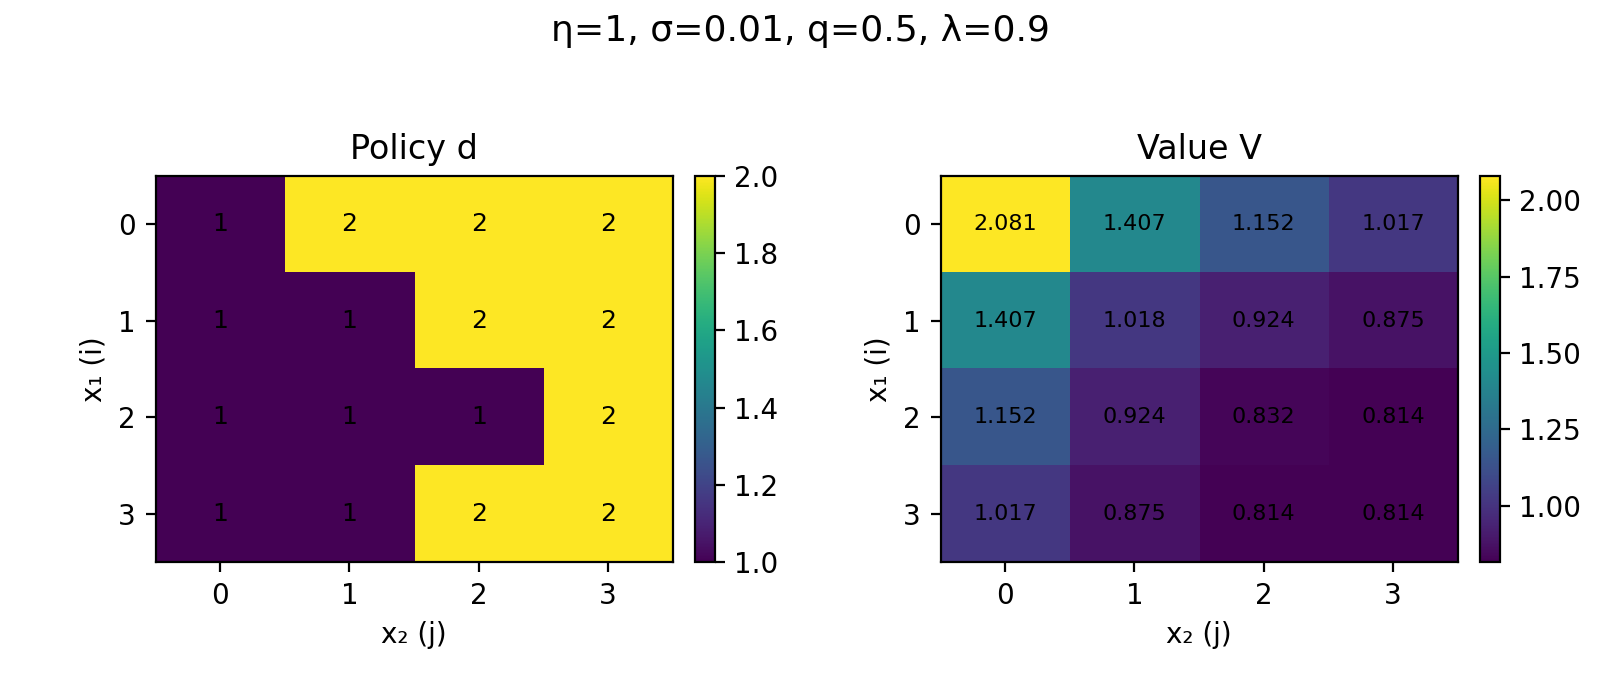
\includegraphics[width=\textwidth]{../aoi_report_plots/eta_1_sigma_0p01_q_0p5_lambda_0p9.png}
\caption{
$\eta=1$, $\sigma=0.01$, $q=0.5$, $\lambda=0.9$\\
Policy and value $v$ (discounted)
}
\end{subfigure}
\vspace{0.5cm}
\begin{subfigure}{0.75\textwidth}
\centering
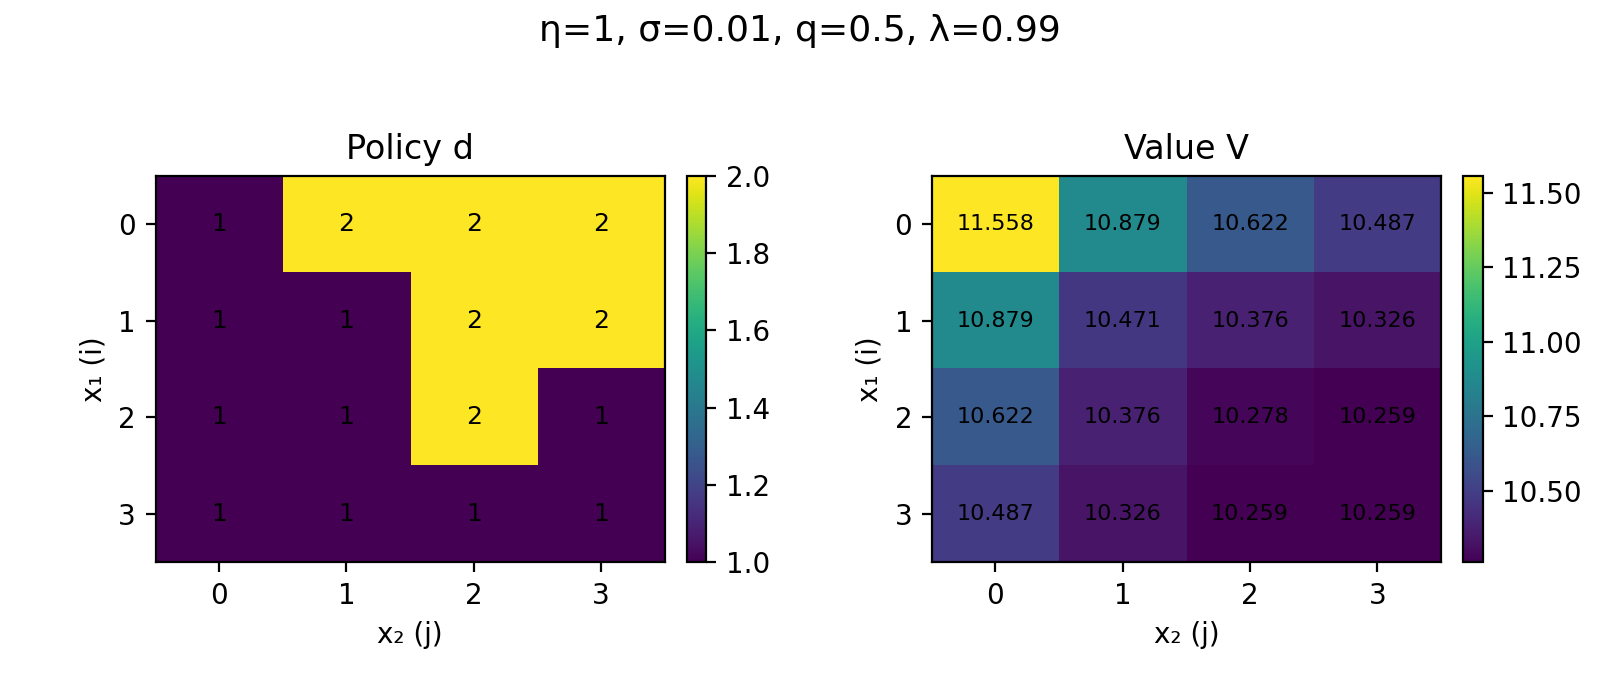
\includegraphics[width=\textwidth]{../aoi_report_plots/eta_1_sigma_0p01_q_0p5_lambda_0p99.png}
\caption{
$\eta=1$, $\sigma=0.01$, $q=0.5$, $\lambda=0.99$\\
Policy and value $v$ (discounted)
}
\end{subfigure}
\caption{Policy and value function for discounted cases ($\lambda = 0.9$ and $\lambda = 0.99$).}
\end{figure}

\begin{figure}[H]
\centering
\begin{subfigure}{0.75\textwidth}
\centering
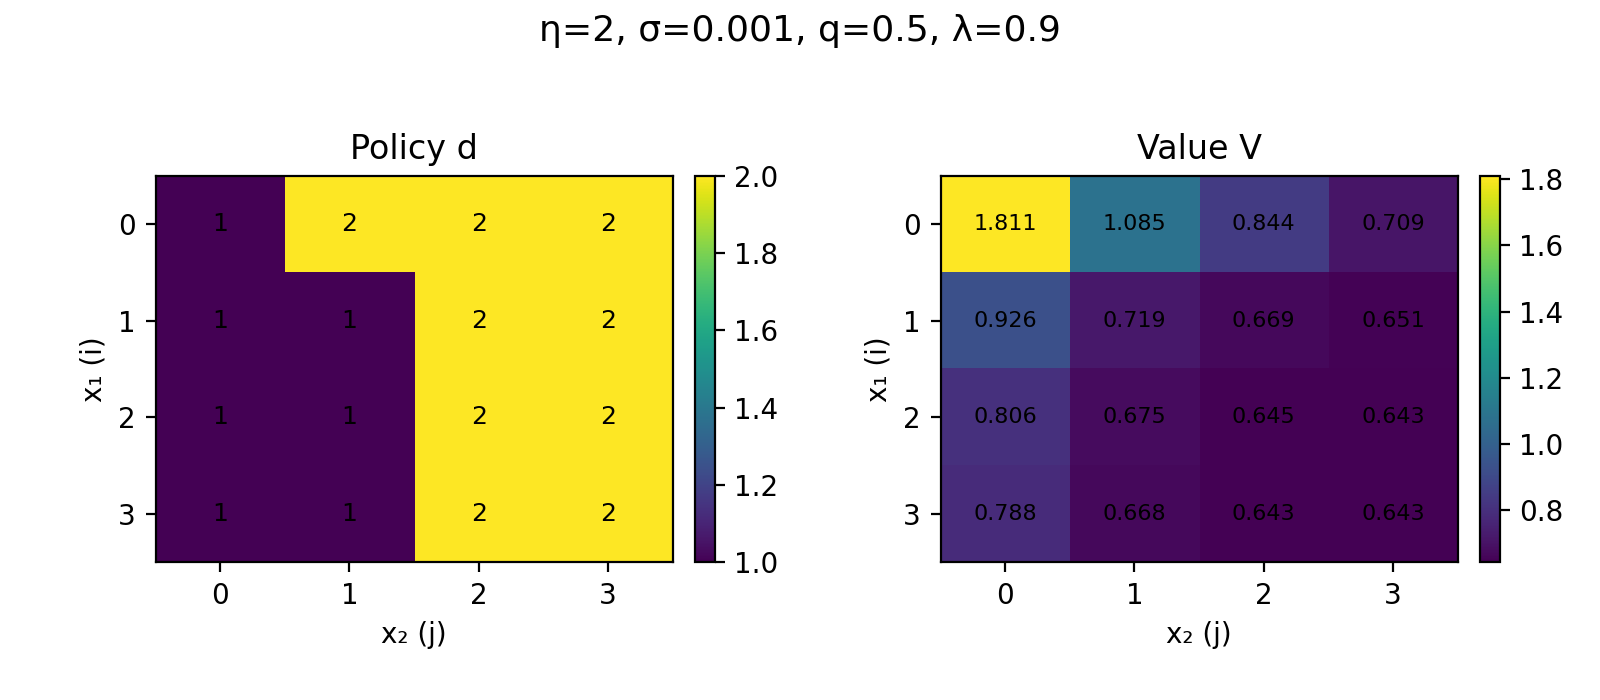
\includegraphics[width=\textwidth]{../aoi_report_plots/eta_2_sigma_0p001_q_0p5_lambda_0p9.png}
\caption{
$\eta=2$, $\sigma=0.001$, $q=0.5$, $\lambda=0.9$\\
Policy and value $v$ (discounted)
}
\end{subfigure}
\vspace{0.5cm}
\begin{subfigure}{0.75\textwidth}
\centering
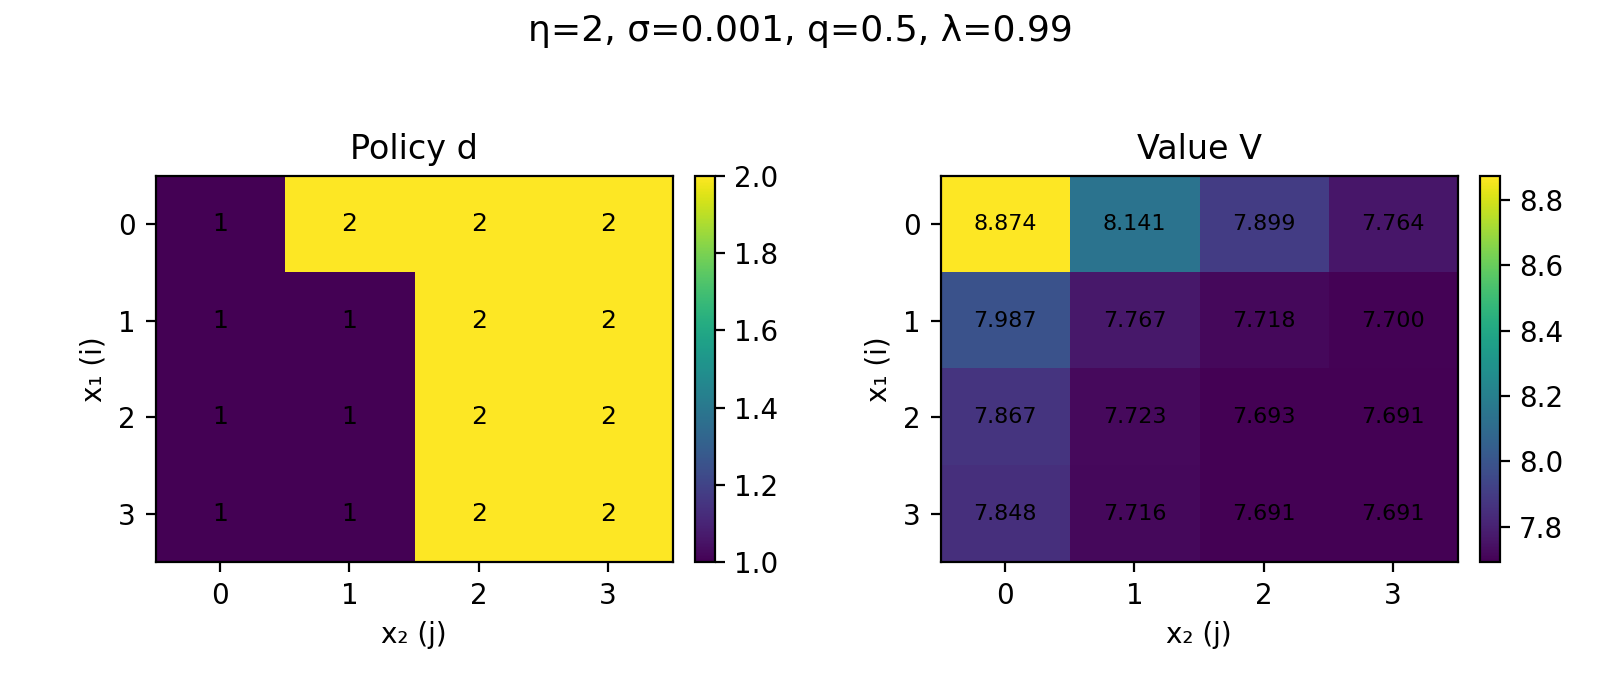
\includegraphics[width=\textwidth]{../aoi_report_plots/eta_2_sigma_0p001_q_0p5_lambda_0p99.png}
\caption{
$\eta=2$, $\sigma=0.001$, $q=0.5$, $\lambda=0.99$\\
Policy and value $v$ (discounted)
}
\end{subfigure}
\caption{Results for a different parameter configuration showing policy and value function for discounted cases.}
\end{figure}

\begin{figure}[H]
\centering
\begin{subfigure}{0.75\textwidth}
\centering
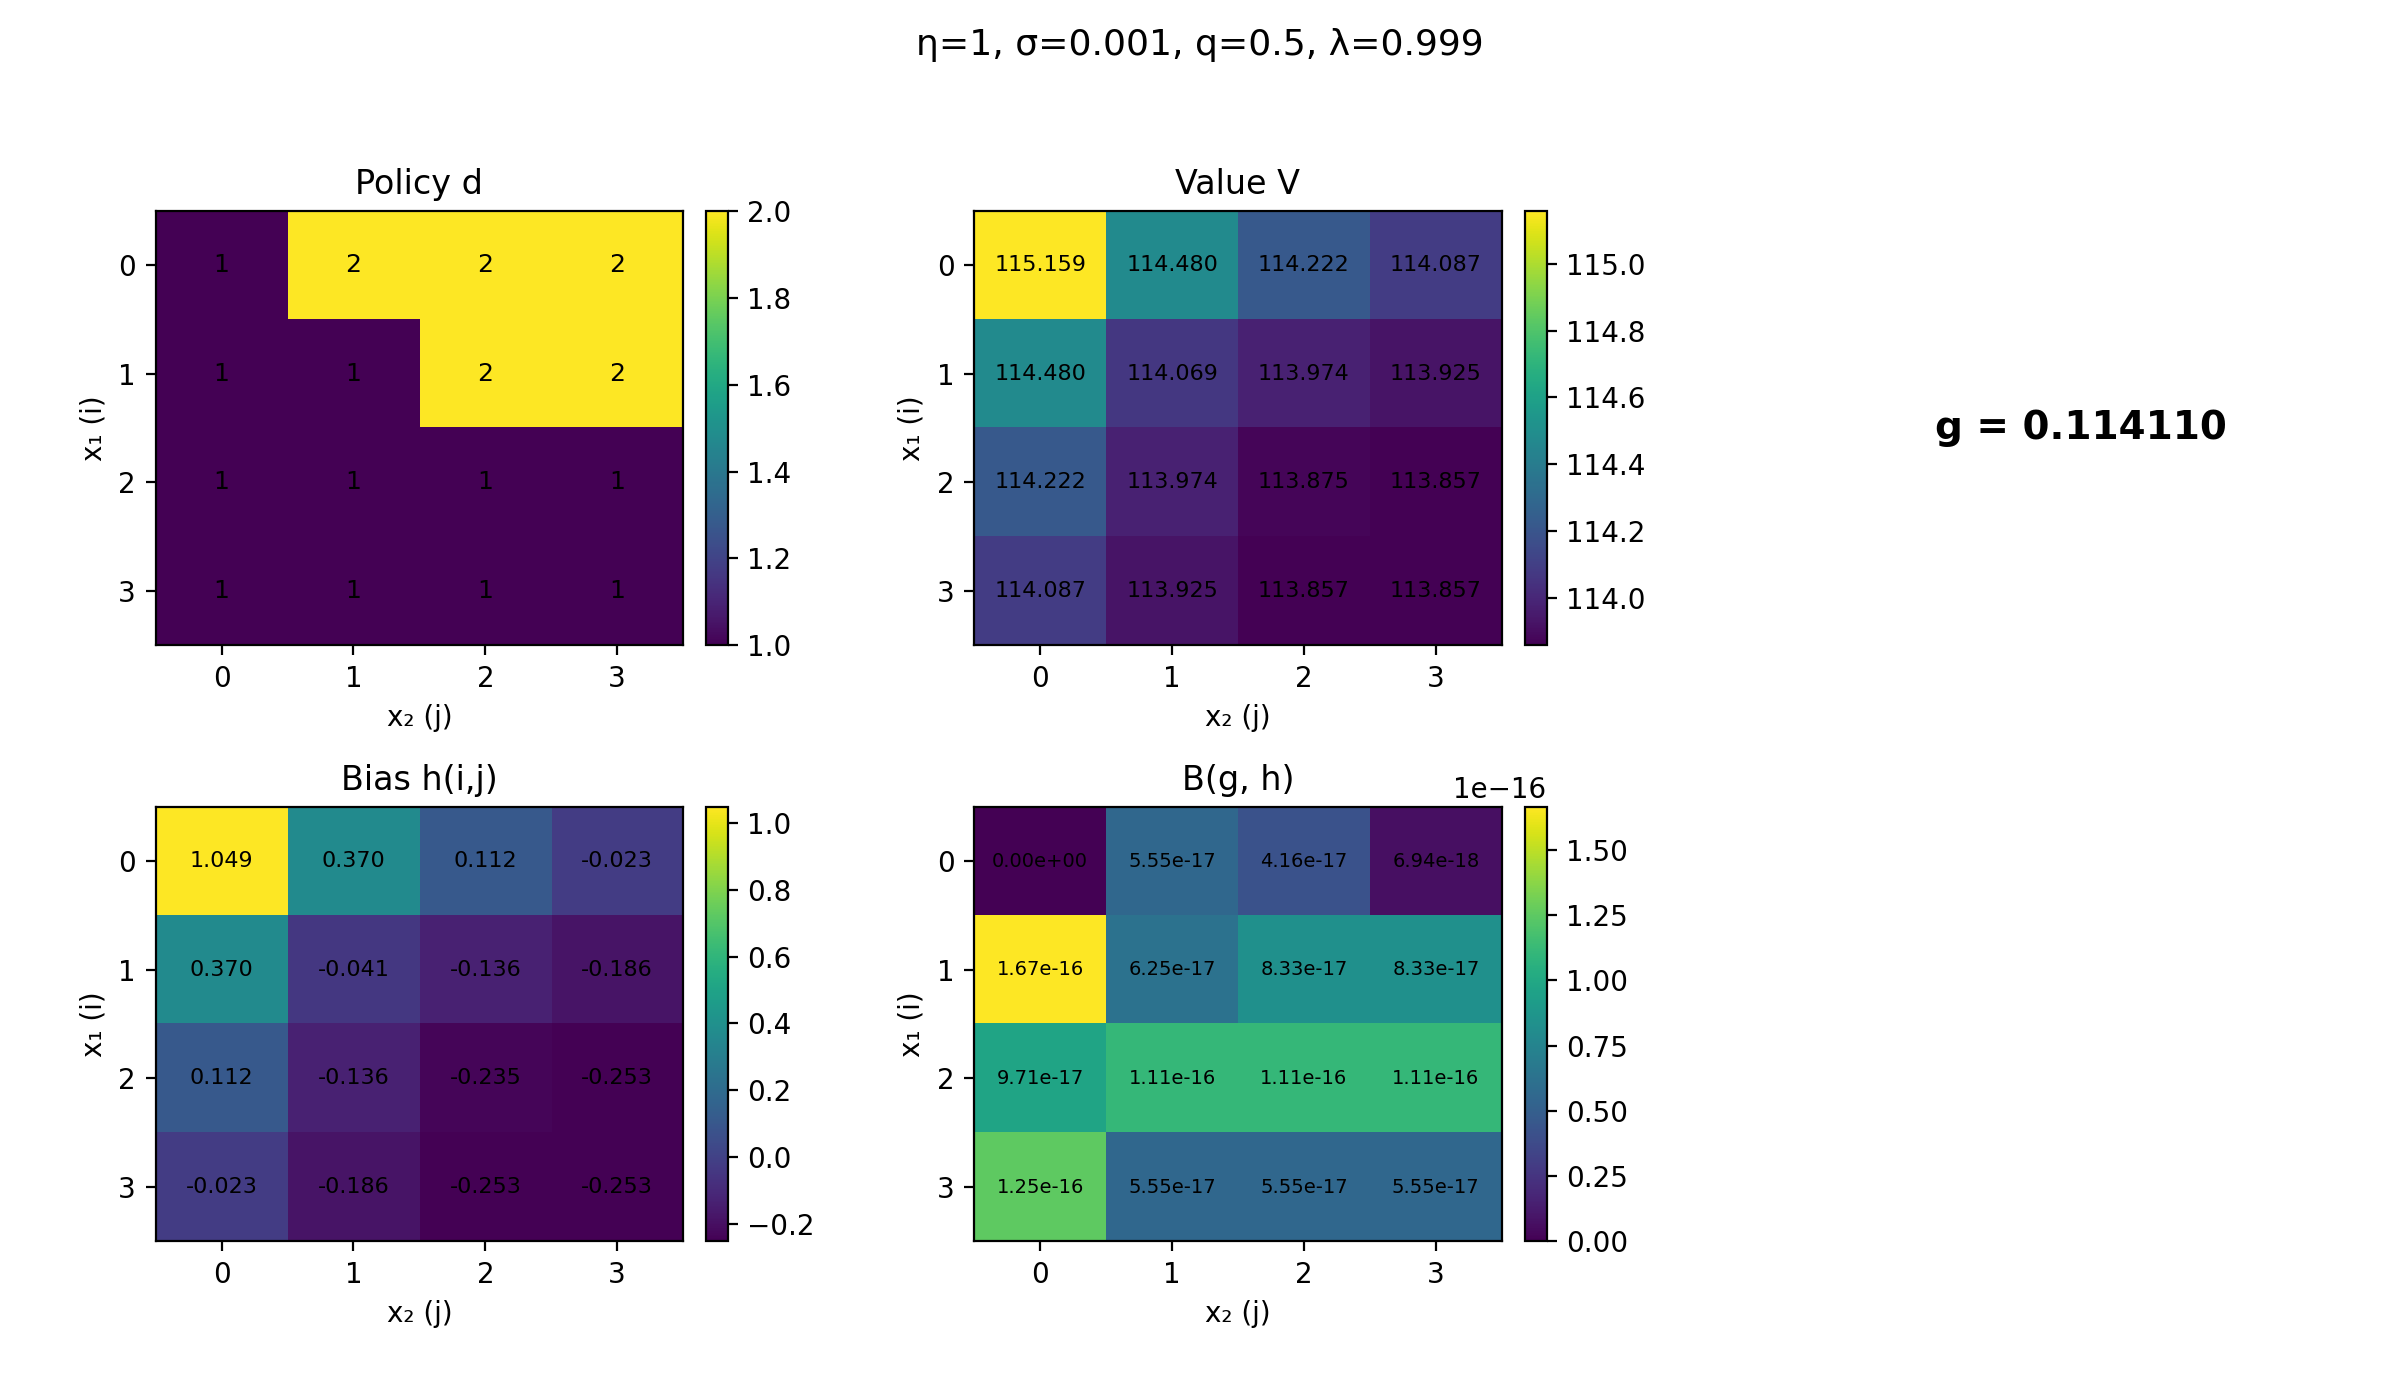
\includegraphics[width=\textwidth]{../aoi_report_plots/eta_1_sigma_0p001_q_0p5_lambda_0p999.png}
\caption{
$\eta=1$, $\sigma=0.001$, $q=0.5$, $\lambda=0.999$\\
All: policy, $v$, $h$, $B(g,h)$, $g$
}
\end{subfigure}
\vspace{0.5cm}
\begin{subfigure}{0.75\textwidth}
\centering
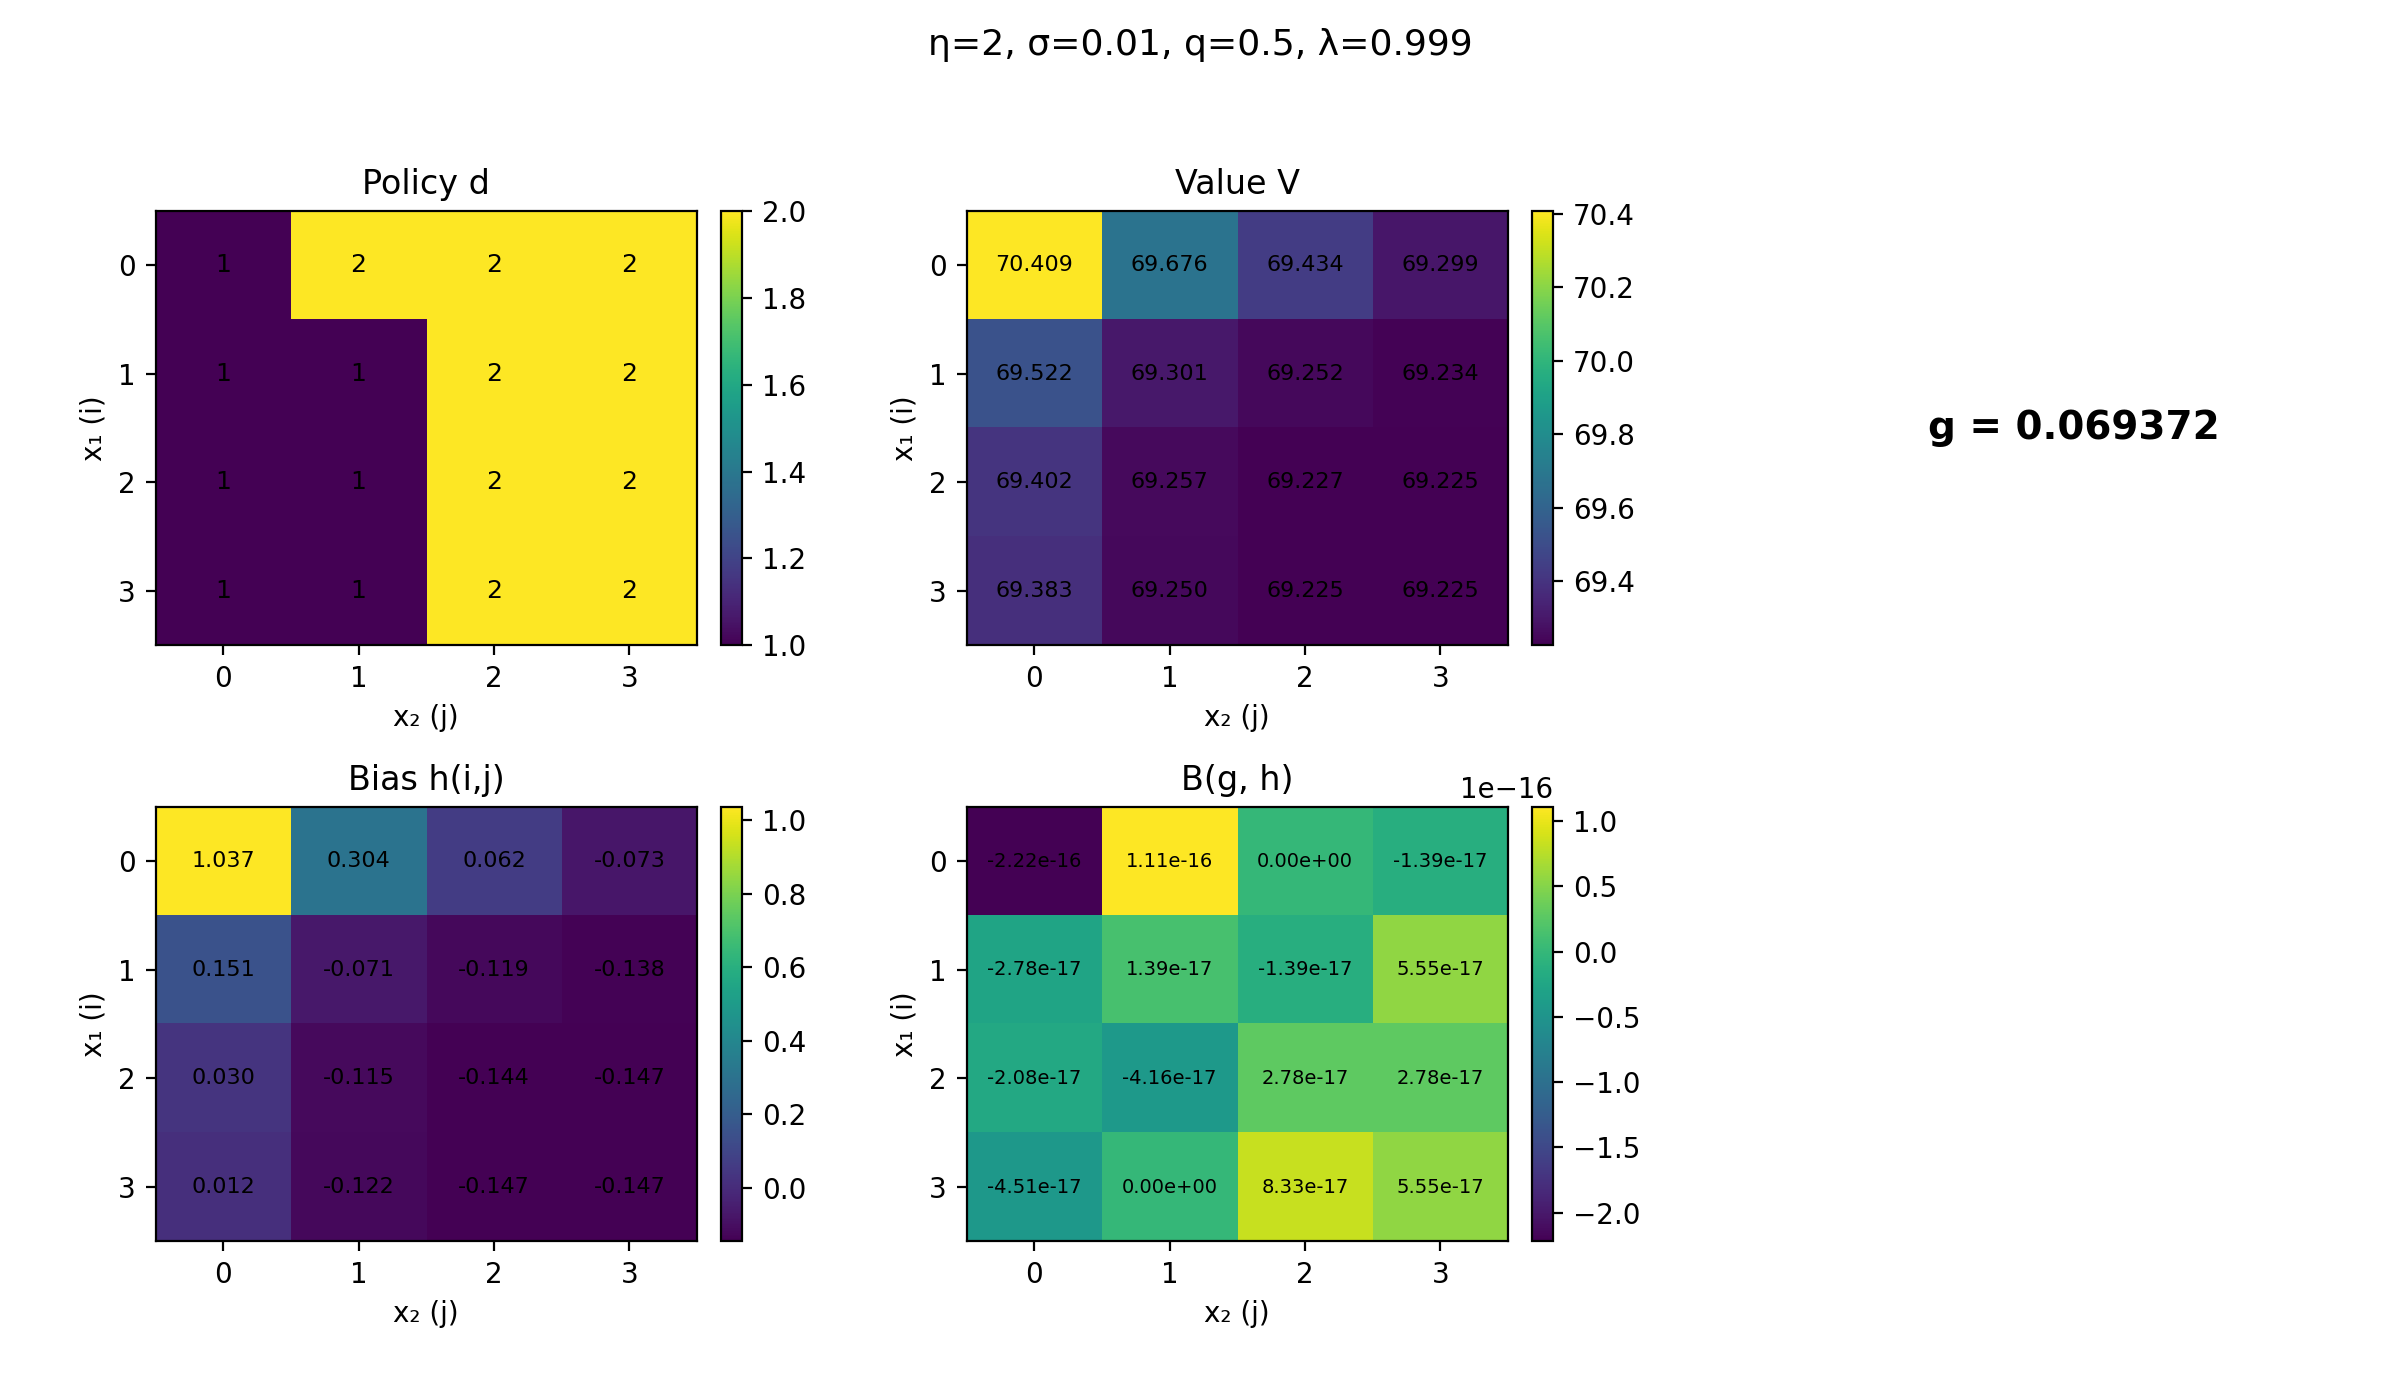
\includegraphics[width=\textwidth]{../aoi_report_plots/eta_2_sigma_0p01_q_0p5_lambda_0p999.png}
\caption{
$\eta=2$, $\sigma=0.01$, $q=0.5$, $\lambda=0.999$\\
All: policy, $v$, $h$, $B(g,h)$, $g$
}
\end{subfigure}
\caption{Average-reward case ($\lambda=0.999$): All relevant metrics are combined in each plot.}
\end{figure}

\section{Unichain Optimality Equations}

When the Bellman error $B(g, h)$ becomes close to 0, the policy satisfies the unichain optimality equations. The unichain optimality equations for an average reward MDP are:

\begin{align}
g + h(s) &= \max_a \left[ R(s, a) + \sum_{s'} T(s'|s, a) h(s') \right] \quad \forall s \in \mathcal{S}
\end{align}


In our numerical experiments with $\lambda = 0.999$ (approaching infinite horizon), we observe that the Bellman error $B(g, h)$ becomes very close to zero across all states, confirming that our computed policies indeed satisfy the unichain optimality equations and are therefore optimal for the average reward criterion.
\section{Comments}
\subsection{Convergence from Discounted to Average Reward}

As the discount factor $\lambda \to 1$, the optimal discounted policy $d_\lambda^*$ converges to the optimal average-cost policy $d^*$.

Mathematically,
$$\lim_{\lambda \to 1^-} d_\lambda^* = d^*.$$

In our numerical results, the policies for $\lambda = 0.999$ coincide with those for smaller $\lambda$ values, confirming this convergence.

\subsection{Unichain Optimality Satisfaction}

For $\lambda = 0.999$, the computed gain $g$ and bias function $h$ satisfy the unichain optimality equations:
$$g + h(s) = \max_a \left[ R(s, a) + \sum_{s'} T(s'|s, a) h(s') \right], \quad \forall s \in \mathcal{S}.$$

The Bellman residual matrix $B(g, h)$ was found to be numerically close to zero:
$$\|B(g, h)\|_\infty \approx 0,$$
confirming that the obtained policy is optimal under the average-reward criterion.

\subsection{Effect of Parameters ($\eta$, $\sigma$, $q$)}

\begin{itemize}
    \item \textbf{Increasing $\eta$} (faster information decay) causes the optimal policy to refresh more aggressively towards 1.
    \item \textbf{Increasing $\sigma$} (higher query cost) discourages querying, resulting in more "wait" (action 0) regions in the policy map.
    \item \textbf{Increasing $q$} (higher success probability) shifts the optimal policy toward more selective querying, as each successful update resets the age more effectively.
\end{itemize}




\end{document}